% -------------------------------------------------------------
%    Implementation
% -------------------------------------------------------------

\section{Implementation}
\subsection{Implementation Frontend}

\subsubsection{Architecture and Technology Stack (MVVM in Avalonia UI)}
\label{sec:architecture-mvvm-avalonia}

The client application is built on the .NET platform using the Avalonia UI framework. Avalonia was chosen for its consistency with the Advanced Object-Oriented Programming course curriculum. The layout is described in XAML, so the structure of the interface is kept in markup files and the C\# code-behind only contains what cannot be expressed declaratively.

The internal structure follows the Model--View--ViewModel (MVVM) pattern. MVVM was selected because the user interface and the optimization logic had to be developed in parallel by two sub-teams, and the pattern enforces a clear boundary between them. Keeping the View independent from the optimization code also made it possible to test the ViewModels in isolation, without instantiating any Avalonia controls. The three layers are organised as follows:

\begin{itemize}
    \item \textbf{View:} The interface is defined in \texttt{MainWindow.axaml}. The file contains only XAML --- layouts, styles, themes and bindings to the corresponding ViewModels. Its code-behind, \texttt{MainWindow.axaml.cs}, is intentionally kept minimal and only handles operations that cannot be expressed through bindings, such as loading the logo asset and switching between the application's pages.

    \item \textbf{ViewModel:} \texttt{MainWindowViewModel.cs} acts as the root ViewModel and owns the nested ViewModels used by the rest of the application. The two main ones are \texttt{DataVisualizerViewModel.cs}, which holds the state and configuration of the interactive charts, and \texttt{UnitViewModel.cs}, which exposes the parameters and operational constraints of an individual heat production unit to the View.

    \item \textbf{Model:} The data layer is represented by the \texttt{DataVisualizerModel.cs} class, which contains time series data, data on previous operations, and data from the optimizer. This class provides access to the data needed for further visualization in the form convenient for use in the ViewModels.
\end{itemize}

Interaction between all three layers in the architecture is provided via the ReactiveUI library. The observable properties of both Models and ViewModels are created using the \texttt{RaiseAndSetIfChanged} method, which raises the property changed event each time the corresponding value changes. Thus, any change in the View, such as changing the slider to maintain a particular heat-producing unit, changes the value in the ViewModel that in turn recalculates the results of the Optimizer and the plot. Therefore, there is no need to explicitly call refreshing in the View.

% DOMINIK
% put your chapters here
\subsubsection{UI Elements and Styling}
The layout of the on-screen UI Elements was designed with the main objective being availability of all functionalities at one place. The operator has access to everything that the system is capable of executing,
from scenario switching, through period switching, to maintenance planning. The entire interface is defined in the MainWindow.axaml file, and it is structured and contained in a Grid container.

The left section - the \textbf{Control Panel} - consists of a dark-red column, 2 radio buttons, slider bar, dropdown menu, and a theme toggle switch. It uses the dark-red coloured background because it is the characteristic color of the \textit{Danfoss} company.
\begin{enumerate}
    \item \textbf{Scenario Switch} - It is built using two rounded radio buttons with the \texttt{GroupName} being "ScenariosGroup". It allows the operator to switch between the Scenario 1 (Heat Scenario)
    and Scenario 2 (Heat \& Electricity Scenario). After selecting an option, the graph in the main section of the frame automatically updates and shows the selected option, either the Heat Scenario
    or the Heat \& Electricity Scenario. The IsChecked binding of this switch is connected to the \texttt{IsHeatScenarioSelected} and the \texttt{IsHeatAndElecScenarioSelected} attributes inside the
    \texttt{MainWindowViewModel.cs} file.
    \item \textbf{Period Switch} - It is also built using two rounded radio buttons with the \texttt{GroupName} being "PeriodGroup". This switch allows the operator to switch between the Summer Period
    and the Winter Period. After selecting an option, the graph in the main section of the frame automatically updates and shows the selected option, either the Summer Period or the Winter Period.
    The \texttt{IsChecked} binding is connected to the \texttt{IsWinterSelected} and the \texttt{IsSummerSelected} attributes inside the \texttt{MainWindowViewModel.cs} file.
    \item \textbf{Maintenance Planning} - Section for scheduling the maintenance period, for time selected using the slider, and for the selected production unit from the dropdown menu. The slider value
    ranges from 30 to 60 hours. In addition, the slider has snapping allowed with the \texttt{TickFrequency} being set to 1. There is a text label under the slider, that is bound to the slider value.
    Furthermore, there is a \texttt{ComboBox} dropdown menu under the text label, containing every production unit available, with the option "None" as well, in case there is no maintenance needed for
    scheduling. The \texttt{SelectedItem} is binded to the \texttt{SelectedUnit} attribute inside the \texttt{MainWindowViewModel.cs} file.
    \item \textbf{Theme Toggle} - A toggle switch located at the very bottom section of the Control Panel sidebar controlling \texttt{IsDarkTheme} and switching the entire system theme.
\end{enumerate}

The right section - the \textbf{Main Section} - consists of 3 vertical areas:
\begin{enumerate}
    \item \textbf{Header} - It consists of a text label stating the official name of the tool, the location/city where the heat distribution is operated at, and the approximate number of buildings in the
    district heating area. In addition, there is a \textit{Danfoss} logo, loaded from the application assets, located at the very right section of the Header.
    \item \textbf{Interactive Chart} - The most important part of the screen. It contains an \texttt{oxy:PlotView}, which is bound to \texttt{Visualizer.CurrentPlotModel}. Below the chart, there is a horizontal
    panel with checkboxes for selecting the metrics to be displayed on the chart, namely: Heat Demand, Heat Production (these two are set to \texttt{IsChecked} as default), Electricity, Electricity Price (these
    two are only available to be selected when operating in the Scenario 2 - the Heat \& Electricity Scenario), CO\textsubscript{2} Eimissions, Fuel Consumption, and the Production Costs). In addition, there
    is a Legend button located in the bottom-right corner of this section, which when clicked expands and displays a detailed pop-up legend, explaining which color on the graph represents what metric.
    \item \textbf{Production Units Cards} - A responsive \texttt{UniformGrid} with three columns, located at the very bottom of the screen below the \textbf{Interactive Chart} section, displaying detailed
    specification of three production units at once. There are arrows located on both left and right side of this section, allowing the operator to navigate between all available production units which are paginated,
    allowing the system to create a new page of production unit cards, in case a unit, or multiple units were added.
\end{enumerate}

To ensure a proffesional interface, there were multiple overrides defined for the \texttt{ControlTemplate} in \texttt{Window.Style}, inside the \texttt{MainWindow.axaml} file. The traditional radio buttons were transformed into a more modern segmented buttons. The following XAML code snippet defines the right-rounded radio button segment with a checkmark visible only when selected:

\begin{figure}[H]
    \centering
    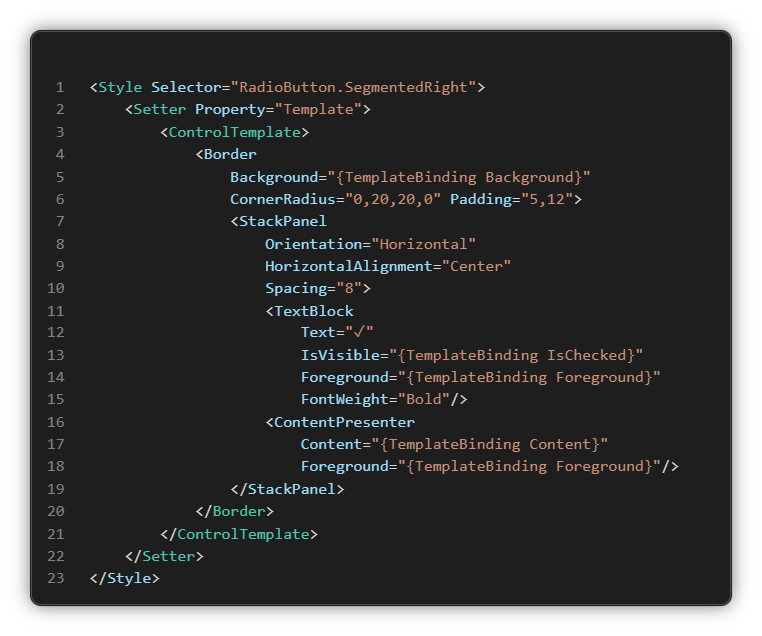
\includegraphics[width=1\textwidth]{Images/RadioButtonStyle.png}
    \caption{Radio Button with Visible Checkmark}
    \label{fig:radiobutton}
\end{figure}

The combo box for selecting production units for maintenance scheduling is also visually customized to have dark-red background, white text, and both hover and selection states.

\begin{figure}[H]
    \centering
    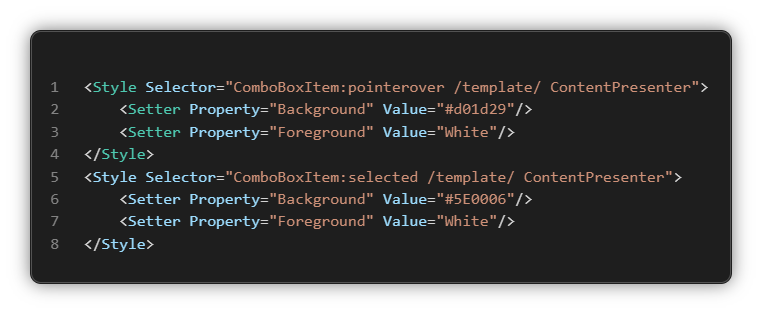
\includegraphics[width=1\textwidth]{Images/ComboBoxStyle.png}
    \caption{Combo Box Style Configuration}
    \label{fig:combobox}
\end{figure}

The production unit cards at the very bottom of the right section are modified rectngular modules (\texttt{CornerRadius="15"}, \texttt{ClipToBounds="True"}). There is the image of the
production unit on the left side of the card, which is loaded from the application assets, and will automatically adapt to the size of the card via \texttt{Stretch="UniformToFill"}.
Lastly, there are specification and different metrics that are significant to each production unit available, and they are shown on the right side of the card. This part of the card is
designed to have dark-red background and white text, which ensures perfect readability even when using lower screen resolutions.

\subsubsection{UI Logic and Engineering Decisions}

\subsubsection{Data Flow}
During the architecture design phase, the main goal of the team was to clearly separate the presentation layer (frontend) from the complex mathematics of the optimisation algorithms (backend). This was achieved by implementing a strict data flow structure.

\begin{enumerate}
    \sloppy
    \item \textbf{Initialisation} 
    
    After the app is launched, \texttt{MainWindow}\allowbreak\texttt{ViewModel} becomes the most important class, since it essentially controls the app flow. This ViewModel requests a list of all available production units using the Asset Manager's \texttt{AssetManager.}\allowbreak\texttt{GetDataForDataVisualizer()} method. In order for the app to load quickly and remain smooth, the \texttt{AssetManager} class is designed to cache all loaded data. When the app is launched for the first time, it uses the \texttt{AssetsLoader} class to read and parse the data from JSON files. Whenever the \texttt{AssetManager} is called again, it does not need to read the data from disk, but rather returns the data directly from the cache. This approach helps to decrease latency as much as possible and ensures that the UI loads more quickly, even with a growing number of production units.

    \item \textbf{Optimisation} 
    
    The optimisation data cycle begins whenever the operator uses the control panel to change the configuration. It can be initiated by either changing the scenario, switching the optimisation period between summer and winter, or adjusting the maintenance settings.
    
    \begin{itemize}
        \item \texttt{MainWindow}\allowbreak\texttt{ViewModel} detects changes in the configuration and launches the \texttt{RefreshData}\allowbreak\texttt{AndChart()} method. This method handles synchronisation of the scenario configuration using the \texttt{ScenarioManager.}\allowbreak\texttt{CurrentScenario} method. Afterwards, the \texttt{SyncOptimization}\allowbreak\texttt{Period()} method is called, which defines clear time boundaries for both the winter and summer periods. The summer period ranges from 8 September to 22 September, while the winter period ranges from 5 January to 19 January. Maintenance settings are sent to the Optimizer module using the \texttt{Optimizer.}\allowbreak\texttt{SetMaintenanceData()} method.
        \item After all configuration data is saved, \texttt{MainWindow}\allowbreak\texttt{ViewModel} instructs \texttt{DataVisualizer}\allowbreak\texttt{Model} to update the data using \texttt{Visualizer.}\allowbreak\texttt{Model.}\allowbreak\texttt{UpdateData()}. At this stage, \texttt{DataVisualizer}\allowbreak\texttt{Model} requests data from \texttt{ResultData}\allowbreak\texttt{Manager}, which starts the optimisation process. The goal of the optimisation is to meet the heat demand using the available production units. The \texttt{Optimizer} calculates workload and then selects the most profitable configuration of units to activate.
        \item When the optimisation process is complete, \texttt{ResultData}\allowbreak\texttt{Manager} saves the result data into CSV files using the \texttt{SaveResultData()} method. These records serve as a debugging tool if the optimisation does not run correctly or for occasional audits.
        \item In the end, the \texttt{DataVisualizer}\allowbreak\texttt{Model} receives the result data in form of \texttt{OptimizedUnit}. It prepares the data for the \texttt{DataVisualizer}\allowbreak\texttt{ViewModel}, where the resulting \texttt{TimeSeries} data are converted into curves and bars on the chart. The \texttt{UpdatePlot()} method links units with the correct colours from \texttt{ChartColors.cs}, sets up axes using \texttt{Axes.cs}, the legend using \texttt{Legend.cs}, and calls \texttt{InvalidatePlot(true)} to ensure that the updated graph is displayed immediately within the GUI.
    \end{itemize}
\end{enumerate}

\vspace{1em}
\noindent\textbf{Conclusion of the Data Flow}

\noindent Due to this strictly engineered data architecture, the entire 14-day optimisation, including exporting data into CSV files and rendering of complex graph usually takes less than 100 milliseconds. The operator therefore receives immediate feedback which ensures a fluid and positive user experience.

